

\begin{alphasection}

\section{Introduksjon - Praktisk rundt filene}

I denne øvingen får dere utlevert noen \verb|.c| og \verb|.h|-filer i \verb|example| og \verb|document_this|-mappene. Tabellen under lister opp alle filene som kommer med i \verb|source|-mappene i de respektive hovedmappene samt litt informasjon om dere skal endre på filene eller om dere skal la dem bli i løpet av øvingen.

\begin{center}
 \begin{tabular}{|p{8.5cm} p{5.5cm}|} 
 \hline
 \textbf{Filer} & \textbf{Skal denne filen endres?}  \\ [0.5ex] 
 \hline\hline
 \verb|example/source/main.c| & nei  \\ 
 \hline
 \verb|example/source/memory_library.c| & nei  \\ 
 \hline
 \verb|example/source/memory_library.h| & nei  \\ 
 \hline
  \verb|document_this/source/main.c| & nei  \\ 
 \hline
 \verb|document_this/source/calculations.c| & nei  \\ 
 \hline
 \verb|document_this/source/calculations.h| & ja  \\ 
 \hline
 \verb|document_this/source/system.c| & nei  \\ 
 \hline
 \verb|document_this/source/system.h| & ja  \\ 
 \hline
\end{tabular}
\end{center}

\section{Introduksjon - Praktisk rundt øvingen}\label{sec:intro}
Dokumentasjon er viktig for videre utvikling av kode. Uten dokumentasjon blir det vanskelig for andre å forstå og bruke koden som har blitt utviklet. Dokumentasjon er særlig viktig når man jobber i en stor gruppe, hvor man som oftest ikke har tid eller trenger å sette seg inn i koden for å kunne implementere og bruke den.

Ulempen med dokumentasjon er at det ikke er særlig gøy. Dermed, hvis kode
og dokumentasjon er separate arbeidsoppgaver, vil dokumentasjonen gjerne
glemmes litt bort. 

Doxygen er en \textit{minste motstands vei} - løsning på dette problemet. Med Doxygen, kan man med spesielt formaterte kommentarer generere dokumentasjon automatisk. Fordelene med å kombinere koding og dokumentasjon med Doxygen er at det da er mer sannsynlig at dokumentasjonen:

\begin{enumerate}
    \item Skrives i utgangspunktet
    \item Oppdateres hver gang koden endrer seg
\end{enumerate}

Til å starte med skal dere få en grunnleggende innføring i bruk av Doxygen i seksjon \ref{sec:2-innføring} med \verb|.c| og \verb|.h|-filene i \verb|example|-folderen. Deretter gjør dere oppgavene i seksjon \ref{sec:3-oppgave} med \verb|.c| og \verb|.h|-filene i \verb|document_this|-folderen for å få godkjent øvingen. 



\section{Introduksjon - Innføring i Doxygen}\label{sec:2-innføring}

Dette kapitlet gir en innføring i bruk av Doxygen med et eksempelprosjekt. Dere har fått utlevert en mappe som heter \verb|example|. I mappen kan dere finne en \verb|memory|-modul, som definerer enkle operasjoner på lister av heltall. Denne modulen er implementert i \verb|memory_library.h| og \verb|memory_library.c|. Prosjekttreet ser slik ut:

\dirtree{%
.1 memory.
.2 Makefile.
.2 source.
.3 main.c.
.3 memory\_library.h.
.3 memory\_library.c.
}


hvor \verb|memory|-modulen består av to funksjoner: \verb|memory_reverse_copy| og\newline \verb|memory_multiply_elements|:
\begin{itemize}
    \item  \verb|memory_reverse_copy| tar inn to buffere, og kopierer fra det første inn i det andre, samtidig som rekkefølgen på elementene blir reversert. 
    \item \verb|memory_multiply_elements| tar inn et buffer som blir skalert med en skaleringsfaktor.
\end{itemize}


\subsection{Konfigurasjonsfil}  

Før man kan bruke Doxygen, må man opprette en konfigurasjonsfil med kommandoen \verb|doxygen -g doxconfig|. Dette er en fil som bestemmer ulike parametre og innstillinger for prosjektet. I dette eksemplet endrer man på disse parametrene:

\verb|PROJECT_NAME = "Memory Library Example"|\newline
\verb|OPTIMIZE_OUTPUT_FOR_C = YES|\newline
\verb|INPUT = source/|\newline
\verb|SOURCE_BROWSER = YES|
\newpage
Prosjekttreet ser nå slik ut:

\dirtree{%
.1 memory.
.2 Makefile.
.2 doxconfig.
.2 source.
.3 main.c.
.3 memory\_library.h.
.3 memory\_library.c.
}

\subsection{Syntaks og kommentering av kode}  

Doxygen genererer dokumentasjon basert på spesielt formaterte kommentarer som består av kommandoer som definerer hvordan kommentaren skal tolkes. For å starte kommandoer i Doxygen bruker man \verb|@|.

Det første Doxygen gjør er å se igjennom kodene etter en \verb|@file|-kommando. Denne \verb|@file|-kommandoen blir definert helt øverst i en fil (\textcolor{RWTHrot100}{\textbf{Ingen \texttt{@file} øverst i koden resulterer i tom dokumentasjon!}}) og melder til Doxygen om at det skal genereres dokumentasjon for denne filen:

\begin{lstlisting}
/**
* @file
* @brief A simple library for doing operations on memory
* buffers consisting of integers
*/
\end{lstlisting}

% \cprotect\framebox{

% \parbox[t][1.75cm]{12.25cm}{
% \addvspace{0.2cm}

% \begin{minipage}{2cm}
%   \dangersign
% \end{minipage}
% \begin{minipage}[c]{10cm}
% Det er lett å glemme at hver fil må ha \texttt{@file} øverst i koden for at dokumentasjon blir generert. Ingen \texttt{@file} resulterer i tom dokumentasjon.
% \end{minipage} 
% } 
% }



I tillegg til \verb|@file|, har man også \verb|@brief| som kort gir en oppsummering av filens funksjon. Doxygen støtter også \textbackslash \ istedenfor \verb|@| for å definere kommandoer. For \verb|C| og \verb|C++| anbefales \verb|@| fordi tegnet ikke kolliderer med \emph{escape characters} (som \textbackslash \verb|n| eller \textbackslash \verb|t|) i koden, og det blir enklere å søke etter Doxygen-kommentarer senere.



\cprotect\subsubsection{\lstinline{int memory_reverse_copy(...)}}
Til og starte med, dokumenterer vi funksjonen \verb|int memory_reverse_copy|. For å dokumentere denne funksjonen, skriver man følgende kommentar inn rett
over \verb|memory_reverse_copy| i \verb|.h|-filen:

\begin{lstlisting}
/**
* @brief Copy a list of integers from one buffer to another,
* reversing the order of the output in the process.
*
* @param[in] p_from Source buffer.
* @param[out] p_to Destination buffer.
* @param[in] size Number of integers in the buffer.
*
* @return 0 on success, 1 if either @p p_from or @p p_to
* is a @c NULL pointer.
*/
\end{lstlisting}

I tillegg til \verb|@brief| som gir en kort oppsummering av hva funksjonen gjør har man \verb|@param| som forteller hva en funksjonsparameter sin oppgave er. Det er også vanlig å legge ved \verb|[in]|, \verb|[out]|, og \verb|[in,out]|. Dette er valgfritt og forteller om parameteren blir modifisert av funksjonen eller ikke. Å bruke \verb|[in]|, \verb|[out]|, og \verb|[in,out]| er spesielt nyttig når man bruker pekere som argument i \verb|C|/\verb|C++|. Følgende konvensjon brukes:

\begin{itemize}
    \item \verb|[in]|: \textit{Input} - parameter som leses og brukes i funksjonen, men som ikke får endret verdi (dvs. blir skrevet til) i funksjonen. 
    \item \verb|[out]|: \textit{Output} - parameter som funksjonen kan endre verdien på men ikke leser og bruker direkte. Dette brukes bare for parametere hvis verdi forblir endret på utsiden av funksjonen etter at denne har returnert (dvs. som regel pekere).
    \item \verb|[in,out]|: \textit{Input} og \textit{Output} - parameteren som lese og brukes direkte i funksjonen, og som kan være endret på utsiden av funksjonen når den returnerer.
\end{itemize}
%\begin{itemize}
    %\item \verb|[in]|: Parameteren er en input til funksjonen og brukes f.eks. i utregninger men får ikke endret sin verdi inne i funksjonen.   
    %\item \verb|[out]|: Parameteren brukes ikke direkte inne i funksjonen, men vil bli endret p̊a utsiden av funksjonen  ̊ar den returnerer.
    %\item \verb|[in,out]|: Verdien til parameteren brukes direkte i funksjonen, og den vil være endret på utsiden av funksjonen når den returnerer.
%\end{itemize}

Kommandoen \verb|@return| dokumenterer hva funksjonen returnerer. Denne trengs ikke om man har en \lstinline{void} - funksjon.

For å legge inn ekstra informasjon i koden bruker man \verb|@c| og \verb|@p|. \verb|@c| er et hint til Doxygen om at det neste ordet er et kodeord. I tilfellet over betyr det at \verb|NULL| blir markert som kode i dokumentasjonen. Likeså, er \verb|@p| et hint til Doxygen om at det neste ordet er en parameter.

Eventuelle kommandoer som Doxygen støtter kan fås ved å ta en titt på\newline \href{https://www.doxygen.nl/manual/commands.html#cmdp}{https://www.doxygen.nl/manual/commands.html\#cmdp}

\cprotect\subsubsection{\lstinline{void memory_multiply_elements(...)}}

For å dokumentere denne funksjonen, skriver man følgenede kommentar inn rett over \verb|memory_multiply_elements| i \verb|.h|-filen:


\begin{lstlisting}
/**
* @brief Multiply all the elements in @p p_buffer, of size
* @p size with the supplied @p factor.
*
* @param[in,out] p_buffer Buffer of integers to be multiplied
* with @p factor.
*
* @param[in] factor Factor to multiply each of the
* elements in @p p_buffer with.
*
* @param[in] size Size of @p p_buffer.
*
* @warning If @p p_buffer is @c NULL, the function will
* abruptly terminate the program with exit code @c 1.
*/
\end{lstlisting}


I tillegg til de overnevnte kommandoene, inkluderer man for denne funksjonen en \verb|@warning| som brukes for å advare brukeren mot oppførsel som ikke er åpenbar. 

\subsection{Automatisk generering av dokumentasjon}  

Dokumentasjon blir automatisk generert ved at man kaller \verb|doxygen doxconfig| i samme mappe som konfigurasjonsfilen. \verb|doxygen doxconfig| generer dokumentasjon både i HTML- og \LaTeX-format, i hver sin mappe. Prosjekttreet ser nå slik ut:
\dirtree{%
.1 memory.
.2 Makefile.
.2 doxconfig.
.2 source.
.3 main.c.
.3 memory\_library.h.
.3 memory\_library.c.
.2 html.
.3 index.html.
.3 [...].
.2 latex.
.3 index.tex.
.3 [...].
}

\verb|GENERATE_LATEX| og \verb|GENERATE_HTML| definert i konfigurasjonsfiguren bestemmer hvilke format Doxygen skal generere dokumentasjon på. I tillegg kan man også spesifisere hvor Doxygen lagrer den genererte dokumentasjonen ved å endre på parameteren \verb|OUTPUT_DIRECTORY|.

Dersom man nå åpner \verb|html/index.html| i en egnet nettleser ved å enten kalle \verb|nettleser html/index.html| fra terminalen, eller trykke \verb|Ctrl + 0| inne i nettleseren og åpne \verb|index.html| derfra blir man møtt av en ganske tom side (se figur \ref{fig:2-dox-fig-main}). Dette er et resultat av at \verb|"related configuration options"| i konfigurasjonsfilen har blitt ignorert i denne øvingen. Opp til venstre hjørne er det en lenke til \verb|Files|, som kan bli fulgt for å få en oversikt som illustrert i figur \ref{fig:2-dox-fig} (se også figur \ref{fig:2-dox-fig2}, \ref{fig:2-dox-fig3}, og  \ref{fig:2-dox-fig4} for dokumentasjon som genereres av doxygen for \verb|memory_library.h|, \verb|int memory_reverse|\verb|_copy|, og \verb|void memory_multiply_elements|).


\begin{figure}[ht]
    \centering
    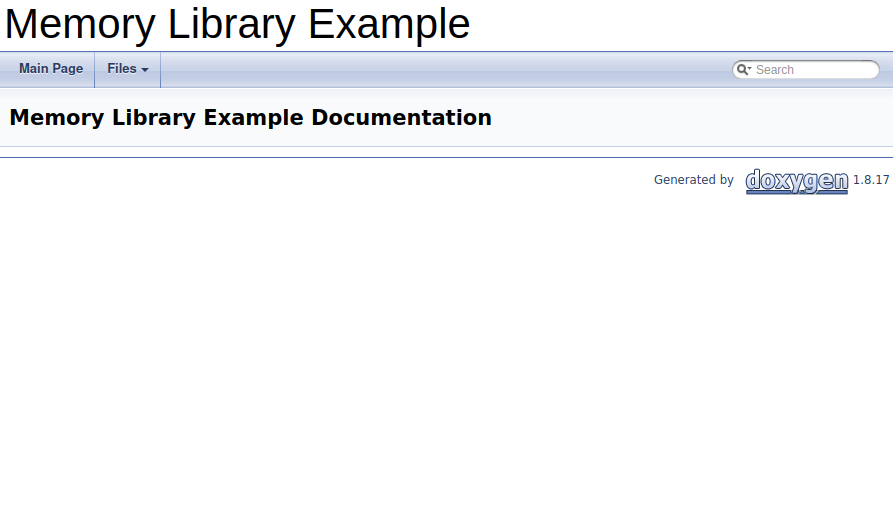
\includegraphics[width=135mm]{figures/doxygen-main.png}
    \caption{Prosjektfilens hovedside.}
    \label{fig:2-dox-fig-main}
\end{figure}

\begin{figure}[ht]
    \centering
    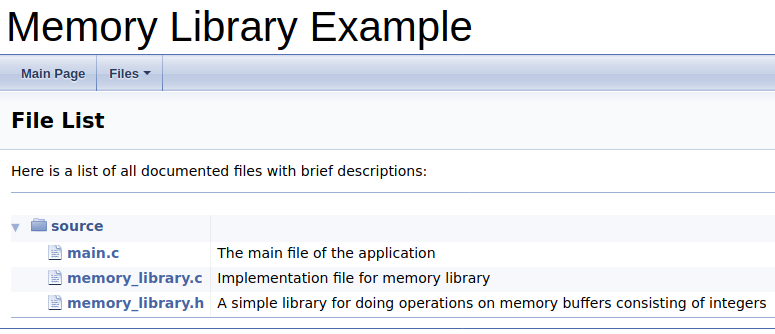
\includegraphics[width=131mm]{figures/doxygenfil1.png}
    \caption{Oversikt over hvilke filer prosjektet består av.}
    \label{fig:2-dox-fig}
\end{figure}


\begin{figure}[H]
    \centering
    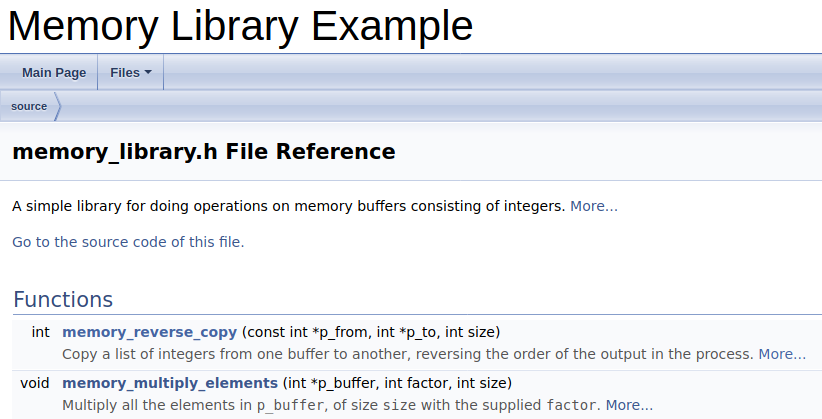
\includegraphics[width=131mm]{figures/doxygenfil2.png}
    \caption{Dokumentasjon for \texttt{memory\_library.h}}
    \label{fig:2-dox-fig2}
\end{figure}

\begin{figure}[H]
    \centering
    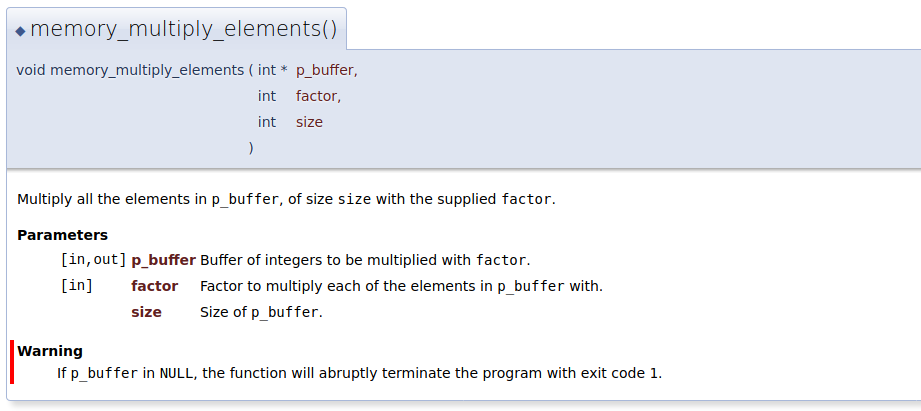
\includegraphics[width=135mm]{figures/doxygenfil3.png}
    \caption{Dokumentasjon for \texttt{int memory\_reverse\_copy}.}
    \label{fig:2-dox-fig3}
\end{figure}



\begin{figure}[H]
    \centering
    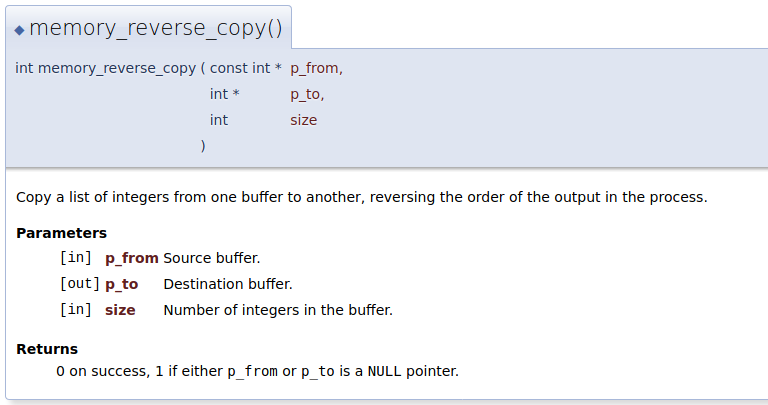
\includegraphics[width=135mm]{figures/doxygen4.png}
    \caption{Dokumentasjon for \texttt{void memory\_multiply\_elements}.}
    \label{fig:2-dox-fig4}
\end{figure}

\end{alphasection}


\setcounter{section}{0}